\chapter{Hardware Umsetzung}

Für die Umsetzung von Wire \& Warriors wurden verschiedene Hardwarekomponenten ausgewählt und integriert. Es sind folgende Komponenten genutzt für die Realisierung:

\textbf{Stepper-Motorn}: Diese Komponenten wurden für die präzisen Bewegungen der Drähte genutzt. Es sind drei Motorn\cite{Tronxy3DPrinter2023} zum Einsatz gekommen: linker Turm, rechter Turm und mittlerer Turm. Dadurch ist es möglich gewesen, die Drähte rotieren zu lassen und die Geschwindigkeit anzupassen.

\textbf{Messingdrähte}: Die Drähte\cite{hagebauGAHALBERTSRundstange2023} sind ein Meter lang gewesen und hatten einen Durchmesser von 6 Millimetern. Die Messingdrähte wurden gewählt, da sie eine gute Balance zwischen Flexibilität und Festigkeit bieten. Zusätzlich besitzt Messing eine gute elektrische Leitfähigkeit, dass ist wichtig gewesen um Berührungen von Spielern zu detektieren.

\textbf{Stepper-Treiber TB6600}: Um die Motorn zu steuern, wurden drei TB6600 Stepper-Treiber\cite{dfrobotTB6600_Stepper_Motor_Driver_SKU__DRI0043DFRobot2023} eingesetzt. Die Treiber ermöglichen die präzise Steuerung der Motorn. Dadurch ist es möglich gewesen, die Motorn gleichmäßig und kontrolliert zu bewegen. Ein enormer Vorteil dieser Treiber ist gewesen, dass sie einfach konfigurierbar durch seitliche Schalter sind. Somit ist es möglich gewesen, die Treiber einfach und schnell auf die Motorn einzustellen.

\textbf{Soundmodul}: Ein Soundmodul ist hinzugefügt worden, um akustisch Feedback für die Spieler zu geben. Dies sollte zur Spielatmospähre beitragen und die Benutzerfreundlichkeit erhöhen.

\textbf{Netzteil}: Es wurde ein Netzteil verbaut, um die Mobilität des Spiels zu gewährleisten. Dadurch kann das Spiel jederzeit flexible an verschiedenen Orten genutzt werden.

\textbf{LEDs}: Es wurden acht LEDs integriert, um visuelles Feedback zu geben. Damit konnten wichtige Spielinformationen wie Spielstatus und die verbleibende Herzen den Spielern angezeigt werden.


\textbf{Arduino Uno-Einsatz}: Dieser Mikrocontroller diente als zentrale Steuereinheit des Spiels. Der Adruino Uno ermöglicht die Steuerung der Stepper-Motoren, das Detektieren von Berührungen und die Ansteuerung der visuellen und akustischen Rückmeldungen durch LEDs und das Soundmodul.

\section{Prototypen}

Mit diesen Komponenten ist es möglich gewesen, das Spiel Wire \& Warrios zu realisieren. Für die ersten Annäherung zur Realisierung des Spieles wurde Prototypen entwickelt. Der erste Prototype sah wie folgt aus:

\begin{figure}[H]
 \centerline{\includegraphics[width=\textwidth,scale=1]{./images/prototype_1.png}}
 \caption{Die Umsetzung des Prototypens zum detektieren von Berürhungen}\label{prototype_1}
\end{figure}

Der erste und simpelste Prototype, wie in der Abbildung \ref{prototype_1} zu sehen, ermöglichte die Detektierung von Berührungen. Die Berührungen wurden durch die rote LED signalisiert. Der nächste Schritt ist gewesen einen Motor einzubauen, um den Draht zu bewegen. Dieser Prototyp sah wie folg aus:


\begin{figure}[H]
 \centerline{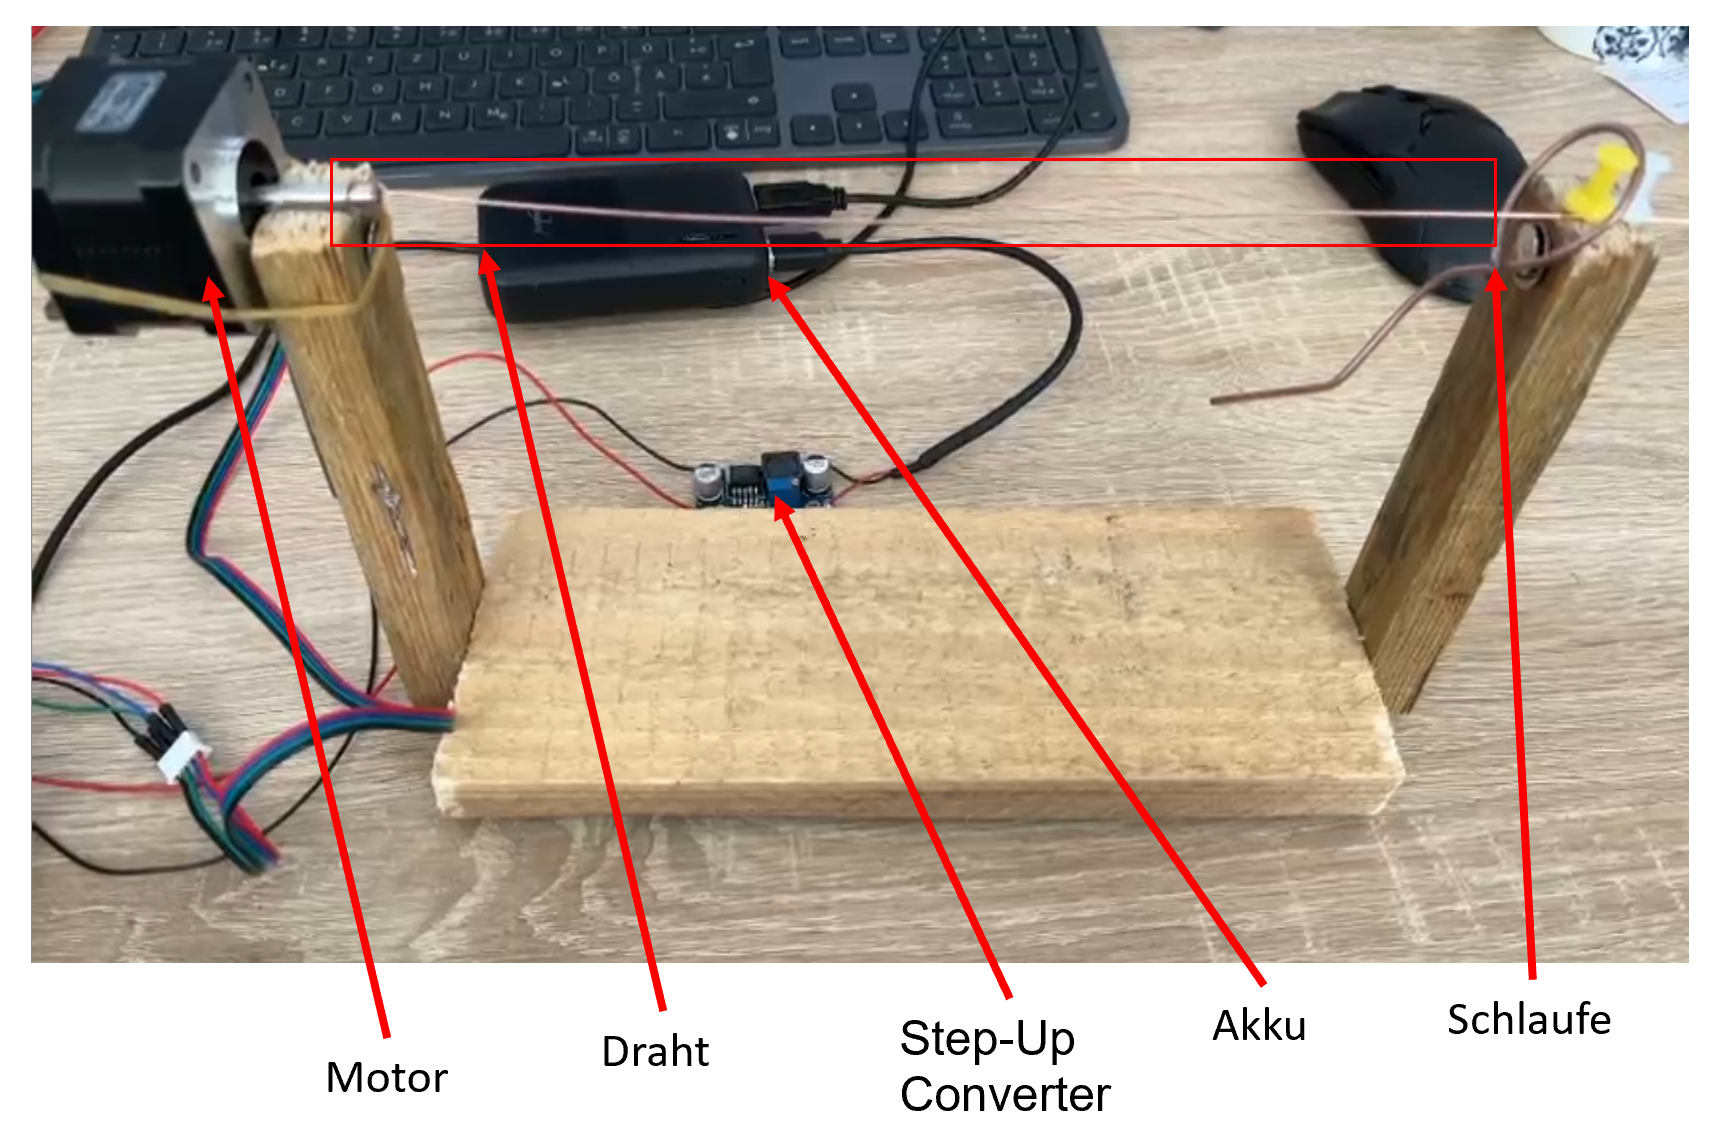
\includegraphics[width=\textwidth,scale=1]{./images/prototype_2.png}}
 \caption{Die Umsetzung des Prototypens}\label{prototype}
\end{figure} 

Mit dem zweite Prototype, in der Abbildung \ref{prototype} zu sehen, ist es möglich gewesen, den Draht zu drehen und Berührungen zu detektieren. Der Step-Up Converter wurde genutzt, um die notwendige Spannung für den Stepper-Motor zu erreichen. Dieser konnte nicht allein durch die Ausgangsspannung vom Akku erreicht werden. Der Step-Up Converter wurde im Endprodukt durch das Netzteil ersetzt.

Zusätzlich musste der Stepper Motor Driver integriert werden, um den Motor zu steuern. Das Schaltbild für die Integrierung sah wie folgt aus:

\begin{figure}[H]
 \centerline{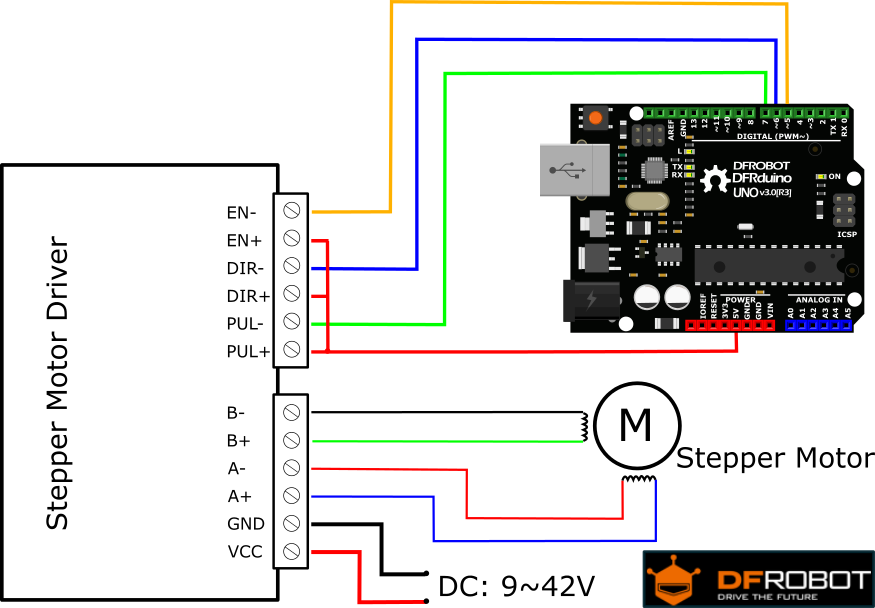
\includegraphics[width=\textwidth,scale=1]{./images/circuit_plan_stepper_motor_driver.png}}
 \caption{Schaltplan des Stepper Motor Drivers}\label{schaltplan_stepper}
 \caption*{Quelle: \href{https://wiki.dfrobot.com/TB6600_Stepper_Motor_Driver_SKU__DRI0043}{TB6600 Stepper Motor Driver}}
\end{figure} 

Der Schaltplan, wie in der Abbildung \ref{schaltplan_stepper} zu sehen, gibt die Verkabelung des Steppers vor. Bevor der Stepper Motor Driver genutzt werden konnte, musste die Stromstärke Konfiguration angepasst werden. Die Stepper Motorn haben eine Stromstärke von 1A benötigt und deshalb mussten die Schalter vier und sechs umgelegt werden. Die Konfigurationen stehen auf dem Stepper Motor Driver und sahen wie folgt aus:

\begin{figure}[H]
 \centerline{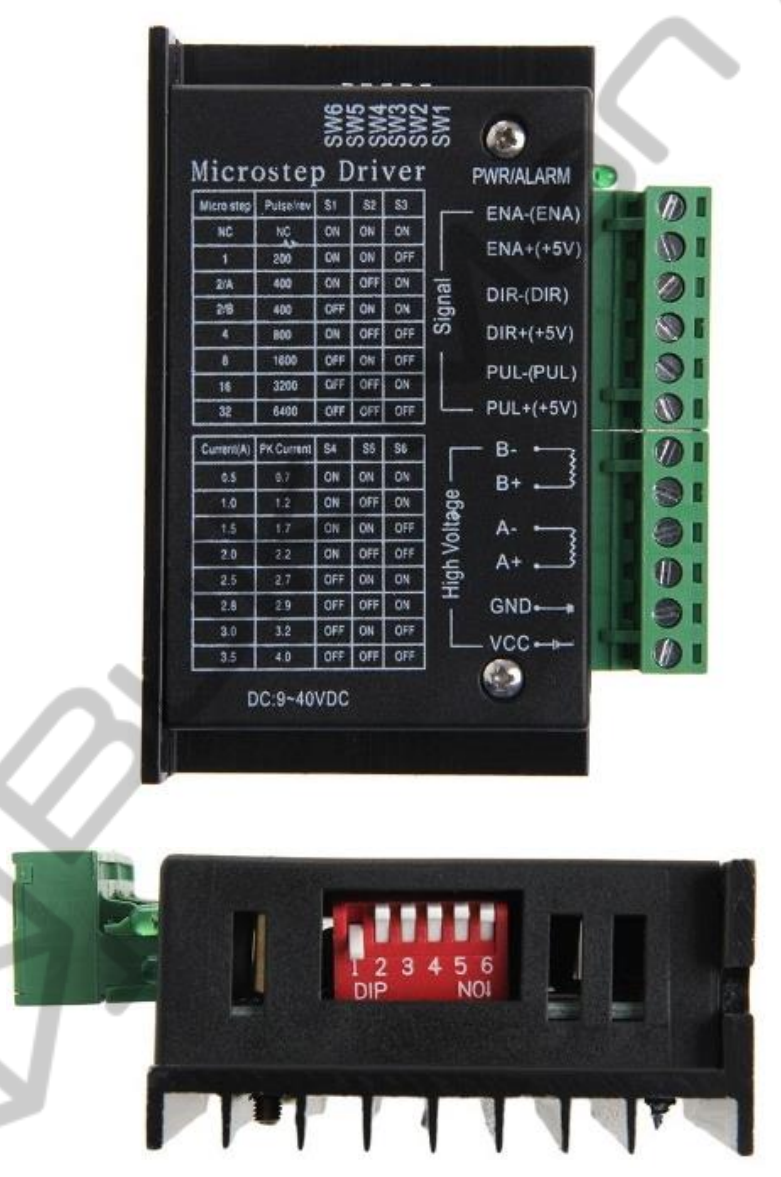
\includegraphics[width=0.45\textwidth,scale=1]{./images/stepper_motor_driver.png}}
 \caption{Konfigurationen auf dem Driver}\label{stepper}
 \caption*{Quelle: \href{https://bulkman3d.com/wp-content/uploads/2019/06/TB6600-Stepper-Motor-Driver-BM3D-v1.1.pdf}{TB6600 Stepper Motor Driver}}
\end{figure} 


Die Ausgänge vom Stepper Driver Motor `EN' und `DIR' wurden nicht genutzt, da die Drähte sich nur eine Richtung drehen sollen. Die Drehung wurde durch Ausgang `PUL' ermöglicht. Die Kabel aus `PUL' wurden am Arduino Uno angebracht.

\section{Realisierung des Projekts}

Das gesamte Gerüst hat eine Länge von einem Meter und eine Breite von 30 Zentimeter. Diese Größe ist kompakt und  bietet eine ausreichend große Spielfläche. Das zusammengebaute Gerüst sieht wie folgt aus:

\begin{figure}[H]
 \centerline{\includegraphics[width=0.25\textwidth,scale=1]{./images/gerüst.jpg}}
 \caption{Gerüst ohne Deckel}\label{turm}
\end{figure} 


Nachdem das Gerüst stand wurden die Türm fertiggestellt und sahen wie folgt aus:

\begin{figure}[H]
 \centerline{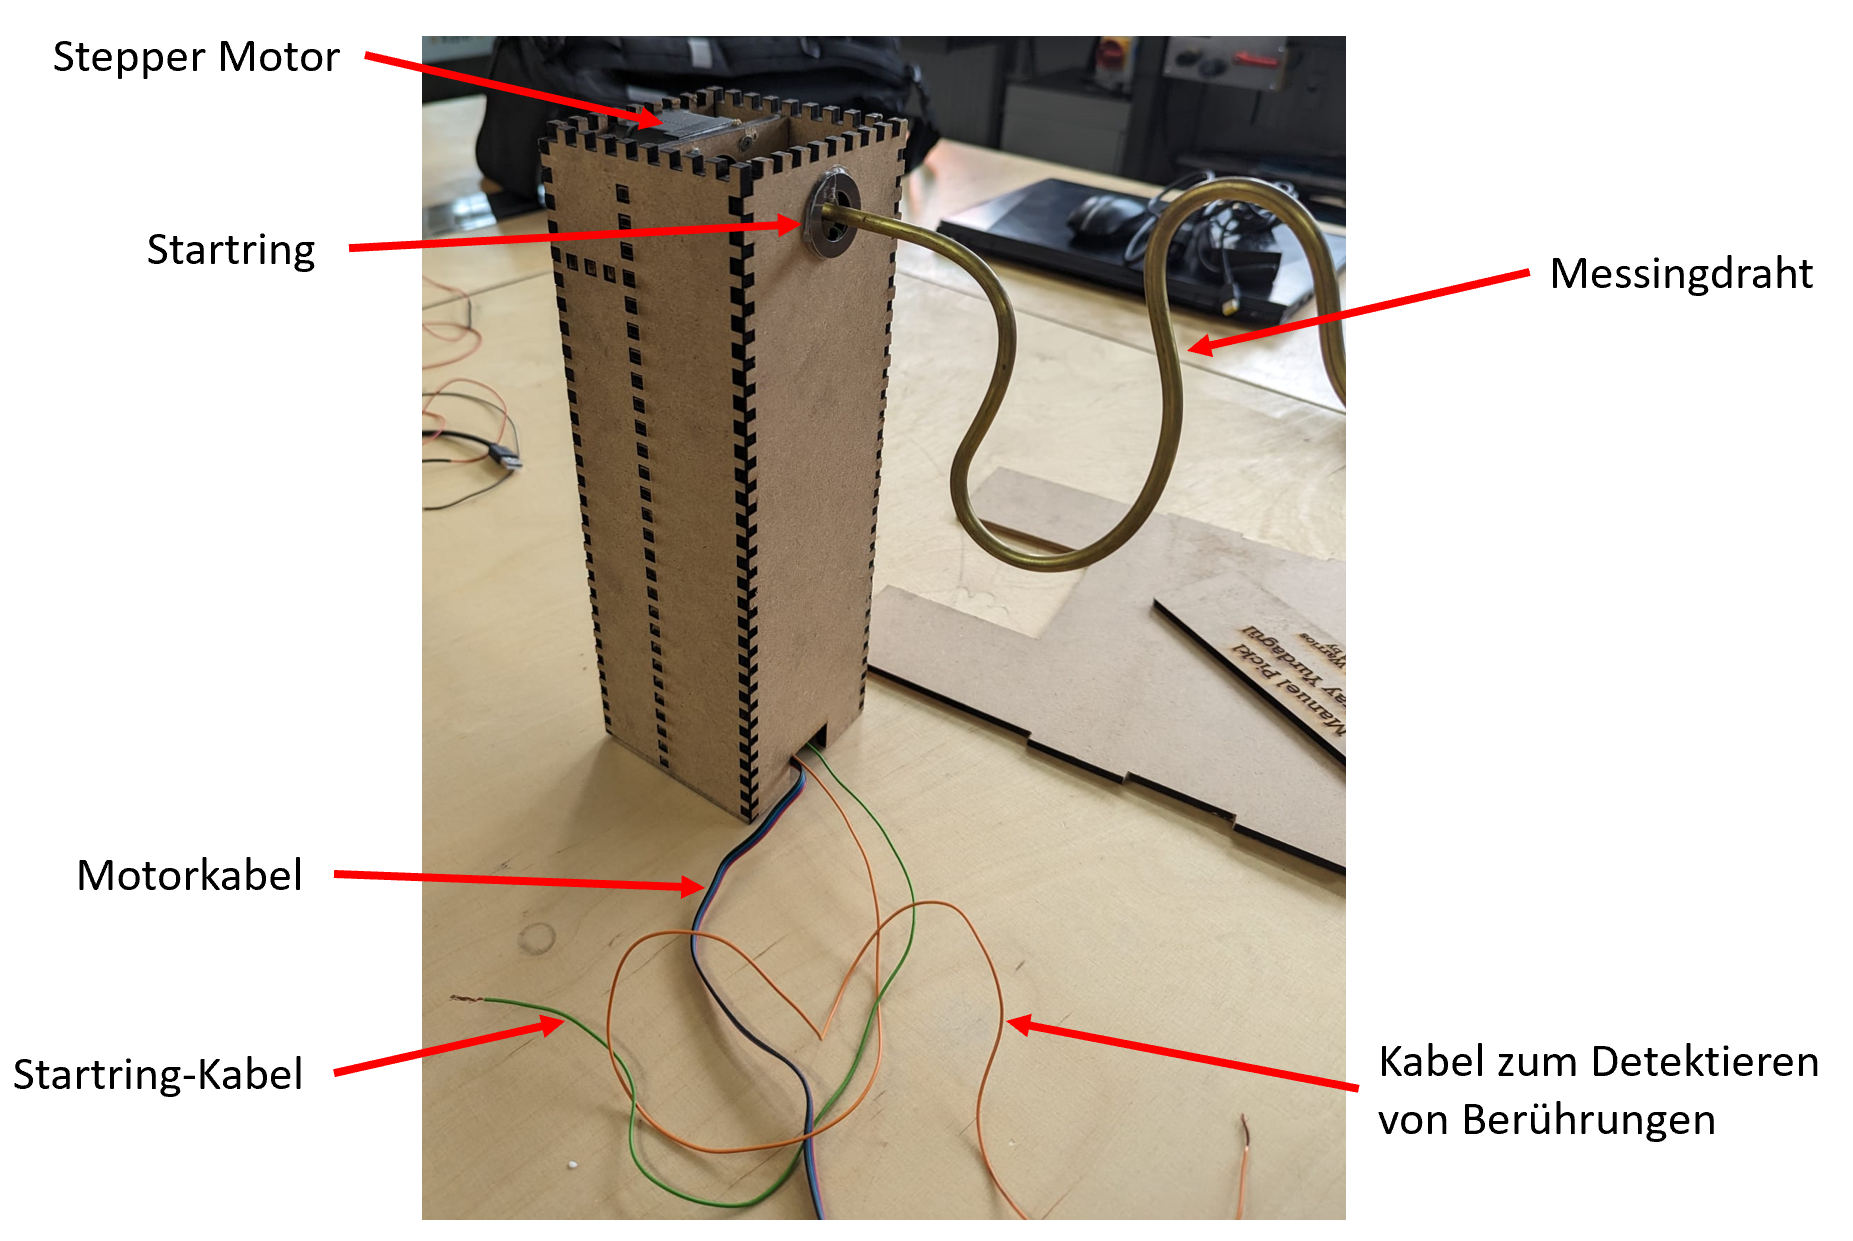
\includegraphics[width=.85\textwidth,scale=1]{./images/turm_holz.png}}
 \caption{Veranschaulichung des fertiggestellt Turms}\label{turm}
\end{figure} 

Die Abbildung \ref{turm} veranschaulicht einen der fertiggestellten Türme. Jeder Turm hat ein Kabel, welches verbunden ist mit dem Draht und eine Ausschnitt am Fuß des Turms für die Kabelführung. Durch die Verbindung mit dem Draht ist es möglich Berührungen zu detektieren. Zusätzlich besitzen die äußeren Türme ein grünes Kabel, welches verbunden ist mit dem Ring am Turm. Damit kann der Spieler signalisieren, dass er sich in der Startposition befindet bzw. das Spiel beenden möchte.

Für die Herz-Anzeige wurden sechs LEDs an einem Gerüst in Reihe montiert und fixiert. Diese Gerüst wurde so konstuiert, sodass es die LEDs direkt unter dem Deckel angebracht werden. Damit ist es möglich gewesen, die herzförmigen Ausschnitt im Deckel des Gerüst optimal zu beleuchten. Dadurch konnten die Spieler genau die verbleibenden Leben sehen und visuelles Feedback erhalten. Das Gerüst sieht wie folgt aus:

\begin{figure}[H]
 \centerline{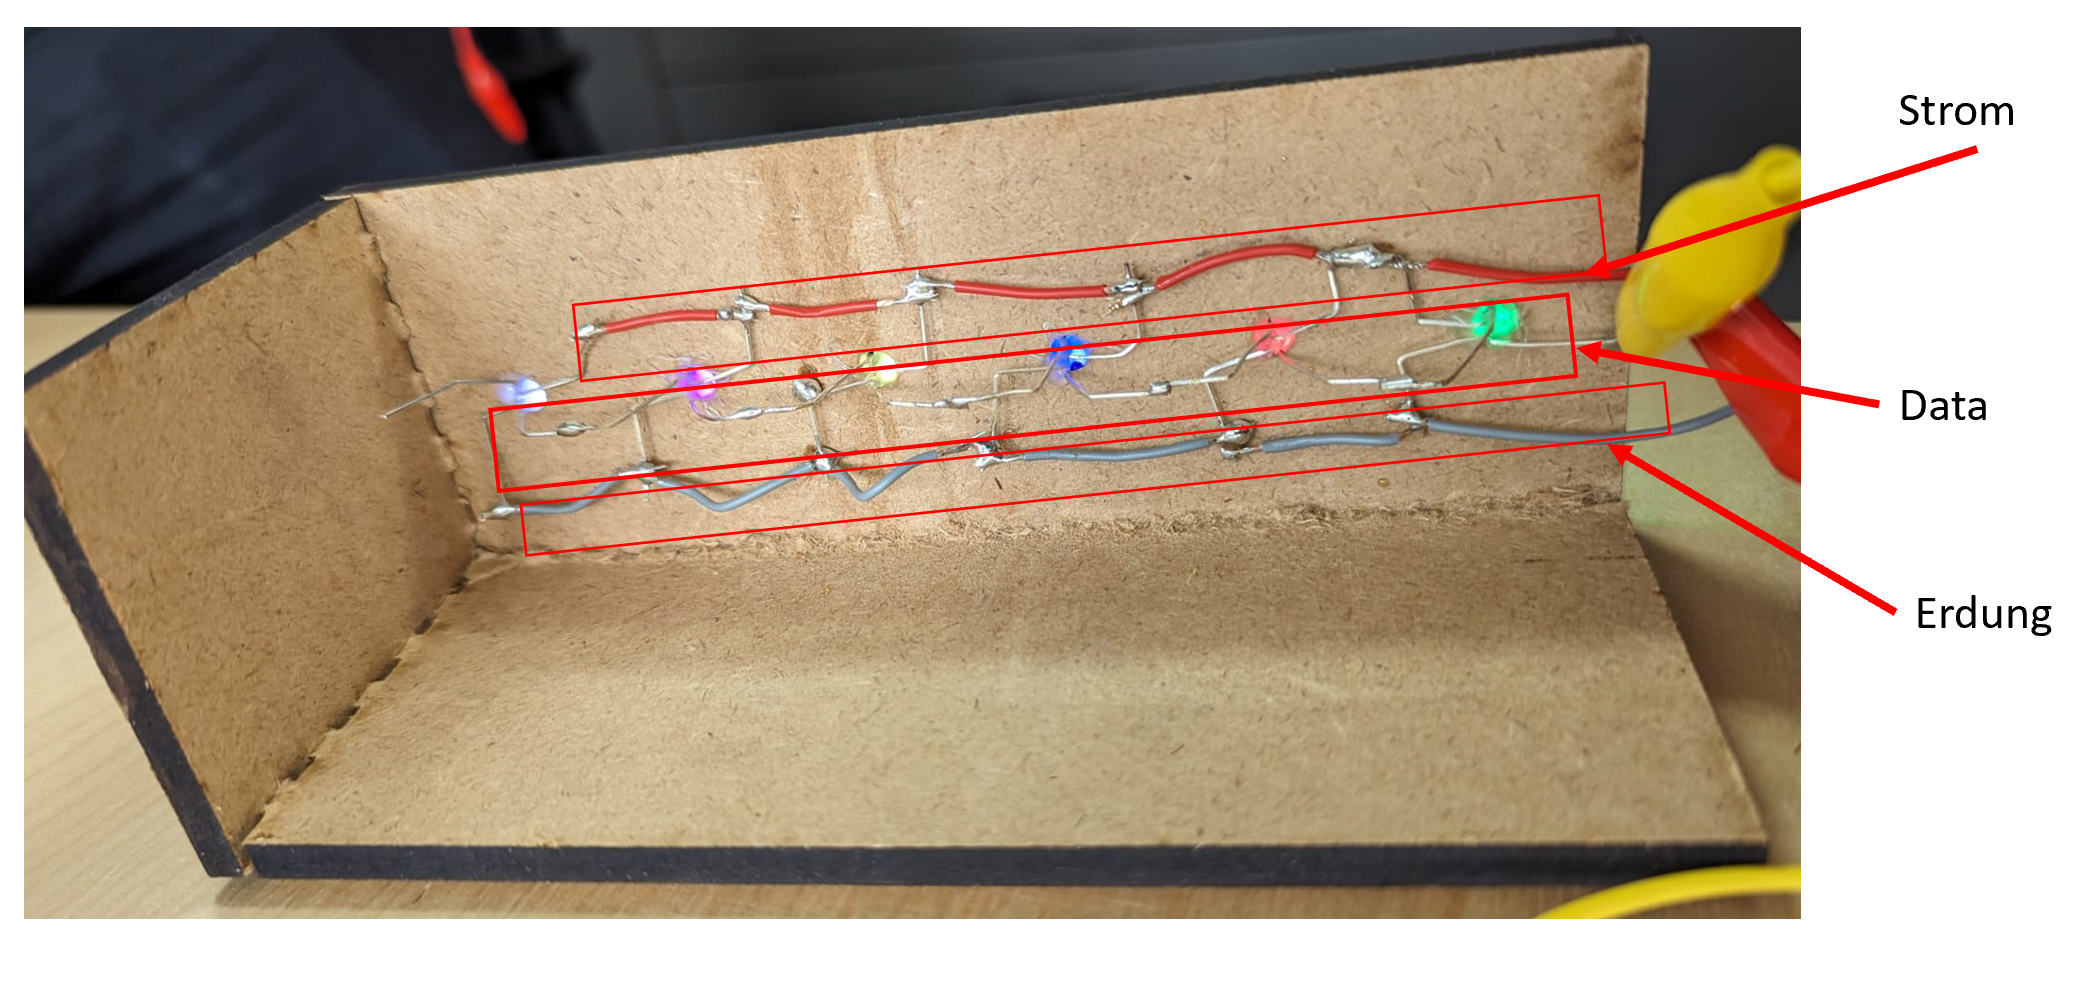
\includegraphics[width=.85\textwidth,scale=1]{./images/herzen_leds.png}}
 \caption{Zusammenlöten der LEDs}\label{herzen}
\end{figure} 

Mit dem erfolgreichen Aufbau der Prototypen und der Implementierung des finalen Gerüsts ist eine solide Basis für das spannende Spielerlebnis von Wire \& Warriors geschaffen worden.